\documentclass[11pt]{article}
\usepackage[utf8]{inputenc}
\usepackage{graphicx}
\usepackage{hyperref}

\title{Notes on Chapter 4 - Functions, Scoping and Abstraction}
\author{Swarup Tripathy \thanks{John V Guttag}}
\date{February 2022}

\begin{document}
    \maketitle
    A curated list of important points for my reference.
    \begin{enumerate}
        \item Parameters inside functions provide something called \textbf{\textit{Lambda Abstraction}}, allowing programmers to write code that manipulates not specific objects
        , but instead whatever objects the caller of the function chooses to use as actual parameters.
        \item In python, there are two ways that formal parameters get bound to actual parameters. 
        \begin{itemize}
            \item The most common method is called the \textbf{positional} -- the first formal parameter is bound to the first actual parameter, the second formal to the second actual
            \item python also supports \textbf{keyword arguments}, in which formats are bound to actuals using the name of the formal parameter.
            \item positional arguments cannot appear after keyword arguments.
        \end{itemize}
        \item Most of the time you will find that you only want to use variables that are local to a function, and the subtleties of scoping will be irrelavant.
        \item Experienced programmers know, however, that an investment in writing testing code often pays big dividends. It certainly beats typing test cases into the shell over and over again during debugging.
        \item Writing help(function name), the system will display the help on the built-in-function.
        \item Abstraction in Python is the process of hiding the real implementation of an application from the user and emphasizing only on usage of it.
        \item Fibonacci's great contribution to European mathematics was his book \textit{Liber Abaci}, which introduced european mathematicians many concepts already well known to Indian and arabic scholars. 
        These concepts included Hindu-Arabic numerals and the decimal system. What we today call the Fibonacci sequence was taken from the work of the \textbf{Sanskrit mathematician Pingala}.
        \item Fibonacci Numbers
        \begin{itemize}
            \item The fib(k - n + 1) will give number of times fib(n) called when calculating fib(k) recursively, where k > n and this works for n = 0 as well.
            \begin{figure}[htp]
                \centering
                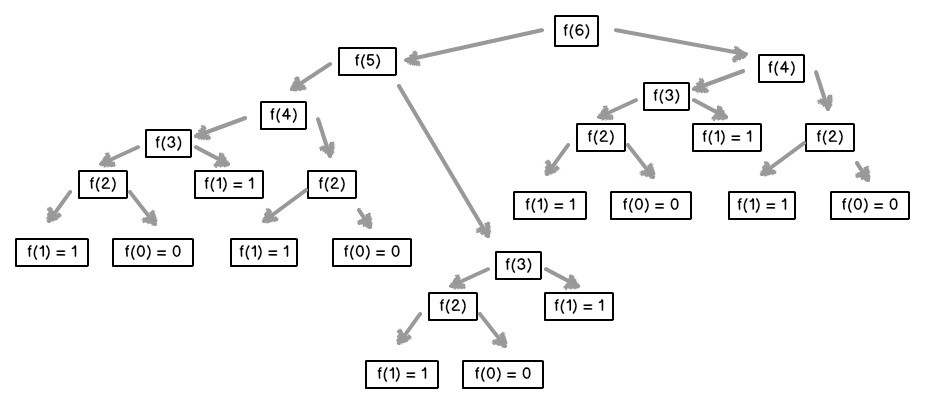
\includegraphics[width=9cm]{imgs/ex1.jpg}
                \caption{An example where k=6 and n=3} \href{https://stackoverflow.com/questions/63136225/how-many-times-does-fib3-gets-called-when-we-call-fib6-using-the-recursive-a}{Reference}.
                \label{fig:galaxy}
            \end{figure}
        \end{itemize}
        \item When two Boolean-valued expressions are connected by 'and', each expression is called a \textbf{conjunct}. If they are connected by 'or', they are called \textbf{disjuncts}.
        \item Fun with Palindromes for Strings
        \begin{itemize}
            \item To check for uppercase and lowercase -> convert to either of them
            \item To check for presence of numbers in between strings which needs to be discarded -> just use for loop having \textbf{in} operator in the alphabets.
            \item If the length of string $\geq$ 1, it's already a Palindrome.
            \item else return s[0]==s[-1] and isPal(s[1:-1]), where s=string and isPal=from-above-point.
        \end{itemize}
    \end{enumerate}
\end{document}